\chapter{Ход работы}
% \addcontentsline{toc}{chapter}{Задание 1. Придумаем}
\label{ch:intro}
\section{Выберем числа}
Для начала выберем четыре целых числа $a, b, c$ и $d$ таким образом, чтобы все они были различными и ни одно из них не равнялось $0$ или $\pm1$.

$a = 2$, $b = 3$, $c = 4$, $d = 5$
\section*{Задание 1. Придумаем матрицы}

\begin{enumerate}
  \item \textbf{Отражение относительно прямой $y = ax = 2x$.}\\
  Обоснование: матрица отражения относительно прямой через начало с углом наклона $\theta=\arctan(a)$ имеет вид
  \[
    R_{y=ax}=\begin{bmatrix}
      \cos 2\theta & \sin 2\theta \\
      \sin 2\theta & -\cos 2\theta
    \end{bmatrix}
    = \frac{1}{1+a^2}\begin{bmatrix} 1-a^2 & 2a \\ 2a & a^2-1 \end{bmatrix}.
  \]
  Для $a=2$ получаем $\cos(2\theta)=\tfrac{1-a^2}{1+a^2}=-\tfrac{3}{5}$, $\sin(2\theta)=\tfrac{2a}{1+a^2}=\tfrac{4}{5}$, откуда
  \[
    M_1 = \begin{bmatrix}
      -\tfrac{3}{5} & \tfrac{4}{5} \\
      \tfrac{4}{5} & \tfrac{3}{5}
    \end{bmatrix}.
  \]

  \item \textbf{Отображение всей плоскости в прямую $y = bx = 3x$.} \\
  Обоснование: столбцы матрицы — образы базисных векторов. Требуем $e_1\mapsto (1,3)^\top$ (любой ненулевой на прямой $y=3x$) и $e_2\mapsto (0,0)^\top$ (схлопывание второй координаты). Тогда
  \[
    M_2 = \begin{bmatrix}
      1 & 0 \\
      3 & 0
    \end{bmatrix}.
  \]

  \item \textbf{Поворот на $10c = 40^\circ$ против часовой стрелки.}\\
  Обоснование: стандартная матрица поворота на угол $\varphi$:
  \[
    M_3 = \begin{bmatrix}
      \cos\varphi & -\sin\varphi \\
      \sin\varphi & \cos\varphi
    \end{bmatrix},\quad \varphi=40^\circ.
  \]

  \item \textbf{Центральная симметрия относительно начала координат.}\\
  Обоснование: $(x,y)\mapsto(-x,-y)$, то есть $M_4=-I$:
  \[
    M_4 = \begin{bmatrix}
      -1 & 0 \\
      0 & -1
    \end{bmatrix}.
  \]

  \item \textbf{Отражение относительно $y = ax$, затем поворот на $10d = 50^\circ$ по часовой стрелке.}\\
  Обоснование: композиция линейных преобразований — произведение матриц справа налево. Пусть $R$ — матрица отражения из п.1, а $P$ — поворот на $-50^\circ$:
  \[
    P = \begin{bmatrix}
      \cos 50^\circ & \sin 50^\circ \\
      -\sin 50^\circ & \cos 50^\circ
    \end{bmatrix},\quad M_5 = P\,R.
  \]

  \item \textbf{Отображение, которое переводит прямую $y = 0$ в $y = ax$ и прямую $x = 0$ в $y = bx$.} \\
  Обоснование: $e_1=(1,0)^\top$ лежит на $y=0$, его образ должен лежать на $y=ax$, возьмём $e_1\mapsto (1,a)^\top$. Аналогично $e_2=(0,1)^\top$ лежит на $x=0$, его образ возьмём на $y=bx$: $e_2\mapsto (1,b)^\top$. Тогда столбцы матрицы — эти образы:
  \[
    M_6 = \begin{bmatrix}
      1 & 1 \\
      a & b
    \end{bmatrix} = \begin{bmatrix} 1 & 1 \\ 2 & 3 \end{bmatrix}.
  \]

  \item \textbf{Отображение, которое переводит прямую $y = ax$ в $y = 0$ и прямую $y = bx$ в $x = 0$.}\\
  Обоснование: требуем, чтобы образы направляющих векторов $v_a=(1,a)^\top$ и $v_b=(1,b)^\top$ лежали соответственно на осях $Ox$ и $Oy$. Искомая матрица $M_7$ удовлетворяет
  \[
    M_7 v_a = (\ast,0)^\top,\quad M_7 v_b = (0,\ast)^\top.
  \]
  Нормировкой можно добиться $M_7 v_a = (1,0)^\top$, $M_7 v_b=(0,1)^\top$, что означает $M_7=[v_a\ v_b]^{-1}$. Явно
  \[
    M_7 = \frac{1}{b-a}\begin{bmatrix} b & 1 \\ -a & 1 \end{bmatrix} = \begin{bmatrix} 3 & 1 \\ -2 & 1 \end{bmatrix}.
  \]

  \item \textbf{Отображение, которое меняет местами прямые $y = ax$ и $y = bx$.}\\
  Обоснование: требуем, чтобы $v_a$ и $v_b$ были собственными направлениями с собственными значениями, меняющими их местами. Достаточно потребовать $M_8 v_a = v_b$ и $M_8 v_b = v_a$. Решая по столбцам, получаем
  \[
    M_8 = \begin{bmatrix} 1 & 0 \\ a+b & -1 \end{bmatrix} = \begin{bmatrix} 1 & 0 \\ 5 & -1 \end{bmatrix}.
  \]

  \item \textbf{Отображение, которое переводит круг единичной площади в круг площади $c = 4$.}\\
  Обоснование: круг $\to$ круг означает изотропное масштабирование с коэффициентом $s=\sqrt{\tfrac{\text{площадь}}{\text{исх. площадь}}}=\sqrt{c}$. Выбираем без дополнительного поворота:
  \[
    M_9 = \sqrt{c}\,I = 2I.
  \]

  \item \textbf{Отображение, которое переводит круг единичной площади в некруг (эллипс) площади $d = 5$.}\\
  Обоснование: эллипс получается при неодинаковом масштабировании по взаимно перпендикулярным осям. Выберем диагональную матрицу с $\det M_{10}=d$ (площадь масштабируется как $|\det|$):
  \[
    M_{10} = \begin{bmatrix} 5 & 0 \\ 0 & 1 \end{bmatrix},\quad \det M_{10}=5=d.
  \]

  \item \textbf{Отображение с перпендикулярными собственными векторами, не лежащими на $y = 0$ или $y = x$.}\\
  Обоснование: вещественная симметричная матрица имеет ортогональный базис собственных векторов (спектральная теорема). Выберем симметричную матрицу с несоосными осями:
  \[
    M_{11} = \begin{bmatrix} 1 & 2 \\ 2 & -1 \end{bmatrix}.
  \]

  \item \textbf{Отображение, у которого нет двух неколлинеарных собственных векторов.}\\
  Обоснование: жорданов блок размера 2 с собственным значением 1:
  \[
    M_{12} = \begin{bmatrix} 1 & 1 \\ 0 & 1 \end{bmatrix}.
  \]

  \item \textbf{Отображение, у которого нет вещественных собственных векторов.}\\
  Обоснование: поворот на $90^\circ$ имеет чисто мнимые собственные значения $\pm i$:
  \[
    M_{13} = \begin{bmatrix} 0 & -1 \\ 1 & 0 \end{bmatrix}.
  \]

  \item \textbf{Отображение, для которого любой ненулевой вектор является собственным.}\\
  Обоснование: это скалярное преобразование $kI$ с $k\neq 0$ — любой вектор сохраняет направление:
  \[
    M_{14} = k I.
  \]

  \item \textbf{Пара отображений, где $AB \neq BA$.}\\
  Обоснование: сдвиги (срезы) вдоль разных осей обычно не коммутируют. Возьмём
  \[
    A = \begin{bmatrix} 1 & 1 \\ 0 & 1 \end{bmatrix},\quad
    B = \begin{bmatrix} 1 & 0 \\ 1 & 1 \end{bmatrix},\quad AB\ne BA.
  \]

  \item \textbf{Пара отображений, где $AB = BA$.}\\
  Обоснование: скалярная матрица коммутирует с любыми, а также коммутируют сдвиги, зависящие от одной и той же оси. В качестве наглядного примера возьмём
  \[
    A = \begin{bmatrix} 1 & 2 \\ 0 & 1 \end{bmatrix},\quad
    B = 3I,\quad AB=BA.
  \]
\end{enumerate}

\section*{Задание 2. Проанализируем}

\textbf{Образы и ядра отображений}

\begin{enumerate}
  \item Матрица $M_1 = 
  \begin{bmatrix}
    -\tfrac{3}{5} & \tfrac{4}{5} \\
    \tfrac{4}{5} & \tfrac{3}{5}
  \end{bmatrix}$\\
  Отражение обратимо ($\det M_1=-1\ne0$), поэтому
  \[
    \mathrm{Range}(M_1) = \mathbb{R}^2,\quad \mathrm{Null}(M_1)=\{\mathbf{0}\}.
  \]

  \item Матрица $M_2 = 
  \begin{bmatrix}
    1 & 0 \\
    3 & 0
  \end{bmatrix}$\\
  \[
    M_2 \begin{bmatrix} x \\ y \end{bmatrix} = \begin{bmatrix} x \\ 3x \end{bmatrix}
    \Rightarrow \mathrm{Range}(M_2)=\{(t,3t)^\top\},\ \mathrm{Null}(M_2)=\{(0,y)^\top\}.
  \]

  \item Матрица $M_{13} = 
  \begin{bmatrix}
    0 & -1 \\
    1 & 0
  \end{bmatrix}$\\
  Поворот обратим, поэтому 
  \[
    \mathrm{Range}(M_{13})=\mathbb{R}^2,\quad \mathrm{Null}(M_{13})=\{\mathbf{0}\}.
  \]

  \item Матрица $M_{14} = k I$, $k\ne0$\\
  \[
    \mathrm{Range}(M_{14})=\mathbb{R}^2,\quad \mathrm{Null}(M_{14})=\{\mathbf{0}\}.
  \]
\end{enumerate}


\textbf{Собственные значения и собственные векторы}

\begin{enumerate}
  \item \textbf{$M_1$}\\
  Характеристический многочлен даёт $\lambda=\pm1$. Для $\lambda=1$ направление отражаемой прямой $y=ax$ сохраняется, для $\lambda=-1$ — ортогональное к ней направление меняет знак. Явно получаем
  $v_{\lambda=1}=(1,2)^\top$, $v_{\lambda=-1}=(2,-1)^\top$.

  \item \textbf{$M_2$}\\
  $\det(M_2-\lambda I)=-(1-\lambda)\lambda \Rightarrow \lambda\in\{0,1\}$. Для $\lambda=1$: $v=(1,3)^\top$; для $\lambda=0$: $v=(0,1)^\top$.

  \item \textbf{$M_3$}\\
  Поворот на $40^\circ$: $\lambda=\cos 40^\circ \pm i\sin 40^\circ$ — вещественных собственных нет.

  \item \textbf{$M_4$}\\
  $\lambda=-1$ кратности 2; любой ненулевой вектор — собственный.

  \item \textbf{$M_8$}\\
  $\lambda=1,-1$, собственные направления — прямые $y=0$ и $x=0$ соответственно.

  \item \textbf{$M_{11}$}\\
  $\det(M_{11}-\lambda I)=\lambda^2-5$, поэтому $\lambda=\pm\sqrt{5}$; собственные векторы ортогональны.

  \item \textbf{$M_{12}$}\\
  Единственное собственное значение $\lambda=1$ с единственным направлением $v=(1,0)^\top$ (дефектная матрица).

  \item \textbf{$M_{13}$}\\
  $\lambda=\pm i$; вещественных собственных векторов нет.

  \item \textbf{$M_{14}$}\\
  $\lambda=k$ кратности 2; любой ненулевой вектор — собственный.

  \item \textbf{$A,B$ из пп.15, 16}\\
  В обоих случаях $\lambda_A=1$, для скалярной $B$ — $\lambda_B=3$ (любой ненулевой вектор собственный).
\end{enumerate}

\textbf{Определители матриц}

\begin{enumerate}
  \item $\det(M_1)=-1$ (отражение).
  \item $\det(M_2)=0$ (сжатие в прямую).
  \item $\det(M_3)=1$ (ортогональная матрица поворота).
  \item $\det(M_4)=1$ (поворот на $180^\circ$).
  \item $\det(M_5)=-1$ (композиция поворота с отражением даёт ориентацию $-$).
  \item $\det(M_9)=4$ (масштаб $2$ по обеим осям).
  \item $\det(M_{10})=5$ (анизотропный масштаб, эллипс той же площади).
\end{enumerate}

\textbf{Где матрица \emph{обязательно} симметрична?}

Матрица \emph{обязательно} симметрична в следующих пунктах задачи (независимо от выбранных представительных матриц внутри класса описанных преобразований):

\begin{enumerate}
  \item[1)] Отражение относительно прямой через начало. Любое такое отражение имеет вид $A=Q\,\mathrm{diag}(1,-1)\,Q^\top$ с ортогональной $Q$, откуда $A=A^\top$.
  \item[4)] Центральная симметрия $A=-I$ — симметрична.
  \item[11)] У матрицы есть два взаимно перпендикулярных собственных направления. В этом случае существует ортонормированный базис из собственных векторов, и матрица ортогонально диагонализуема: $A=Q D Q^\top$, следовательно симметрична.
  \item[14)] Скалярная матрица $A=kI$ — симметрична.
\end{enumerate}

В остальных пунктах симметричность не является обязательной: например, в п.9 круг в круг можно переводить с дополнительным поворотом $A=sR$ (не симметрична при $R\ne\pm I$), а в п.10 эллипс можно получить композицией двух разных поворотов с диагональным масштабом $A=R_1 \mathrm{diag}(\alpha,\beta) R_2$.

\section*{Визуализация линейных отображений}

\begin{figure}[H]
  \centering
  \begin{subfigure}[b]{0.3\textwidth}
    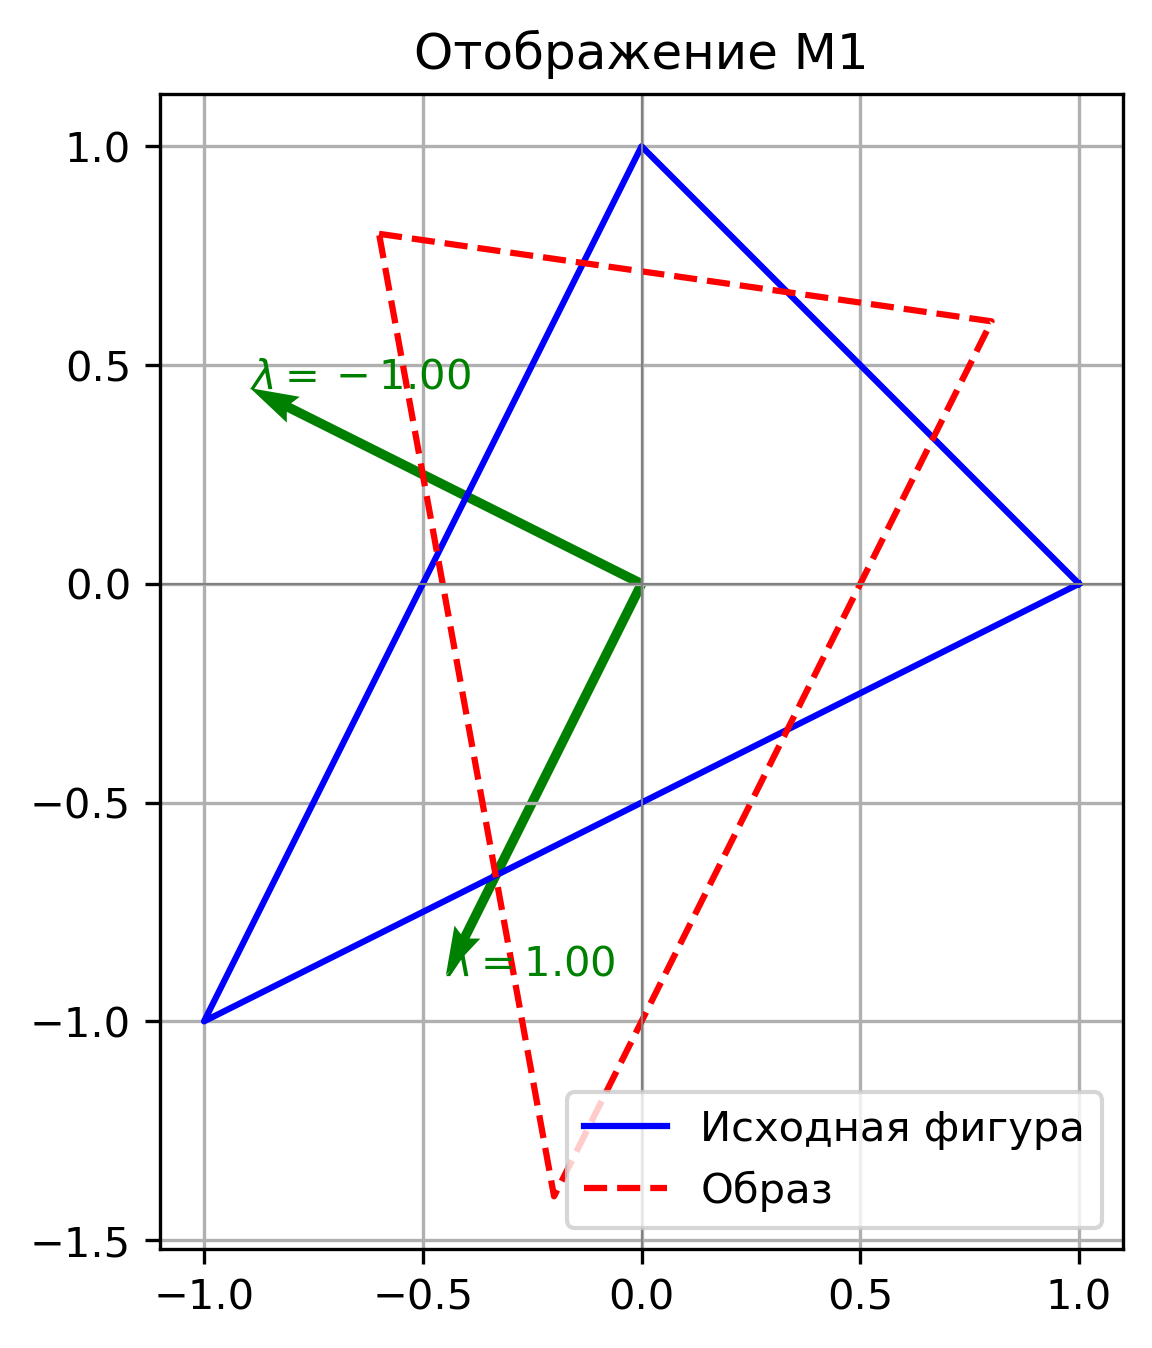
\includegraphics[width=\linewidth]{plots/M1.png}
    \caption{$M_1$}
  \end{subfigure}\hfill
  \begin{subfigure}[b]{0.3\textwidth}
    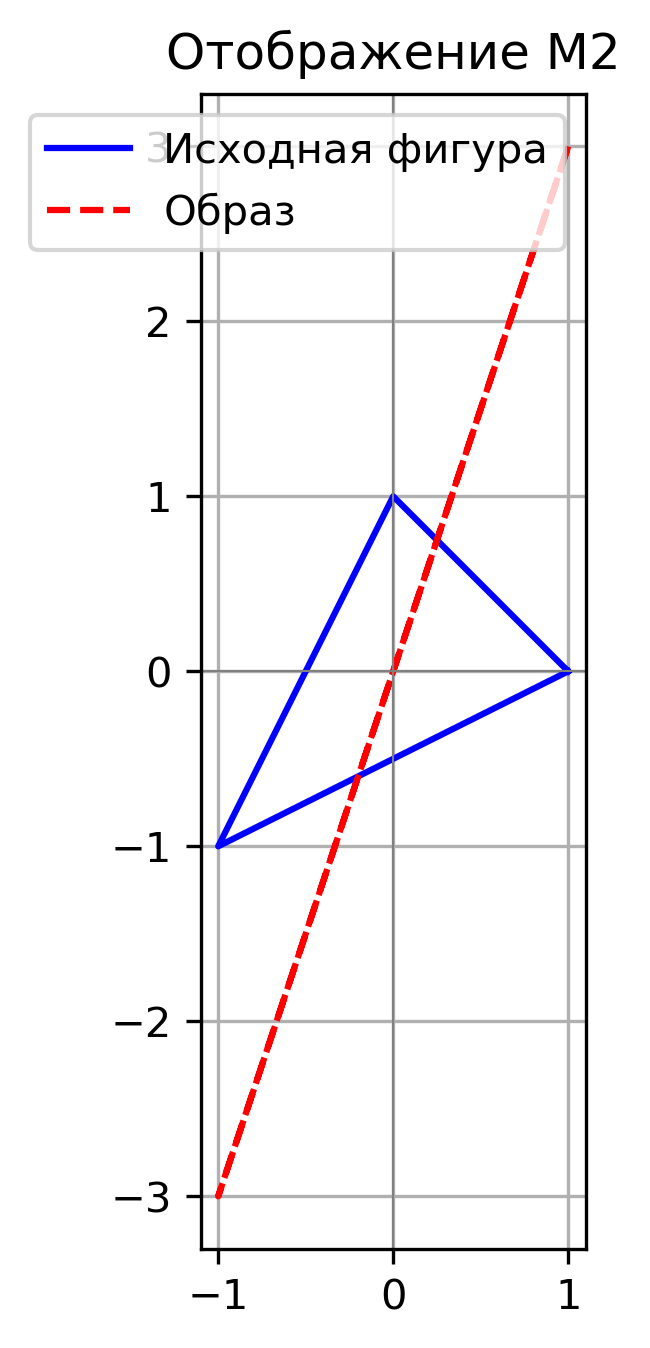
\includegraphics[width=\linewidth]{plots/M2.png}
    \caption{$M_2$}
  \end{subfigure}\hfill
  \begin{subfigure}[b]{0.3\textwidth}
    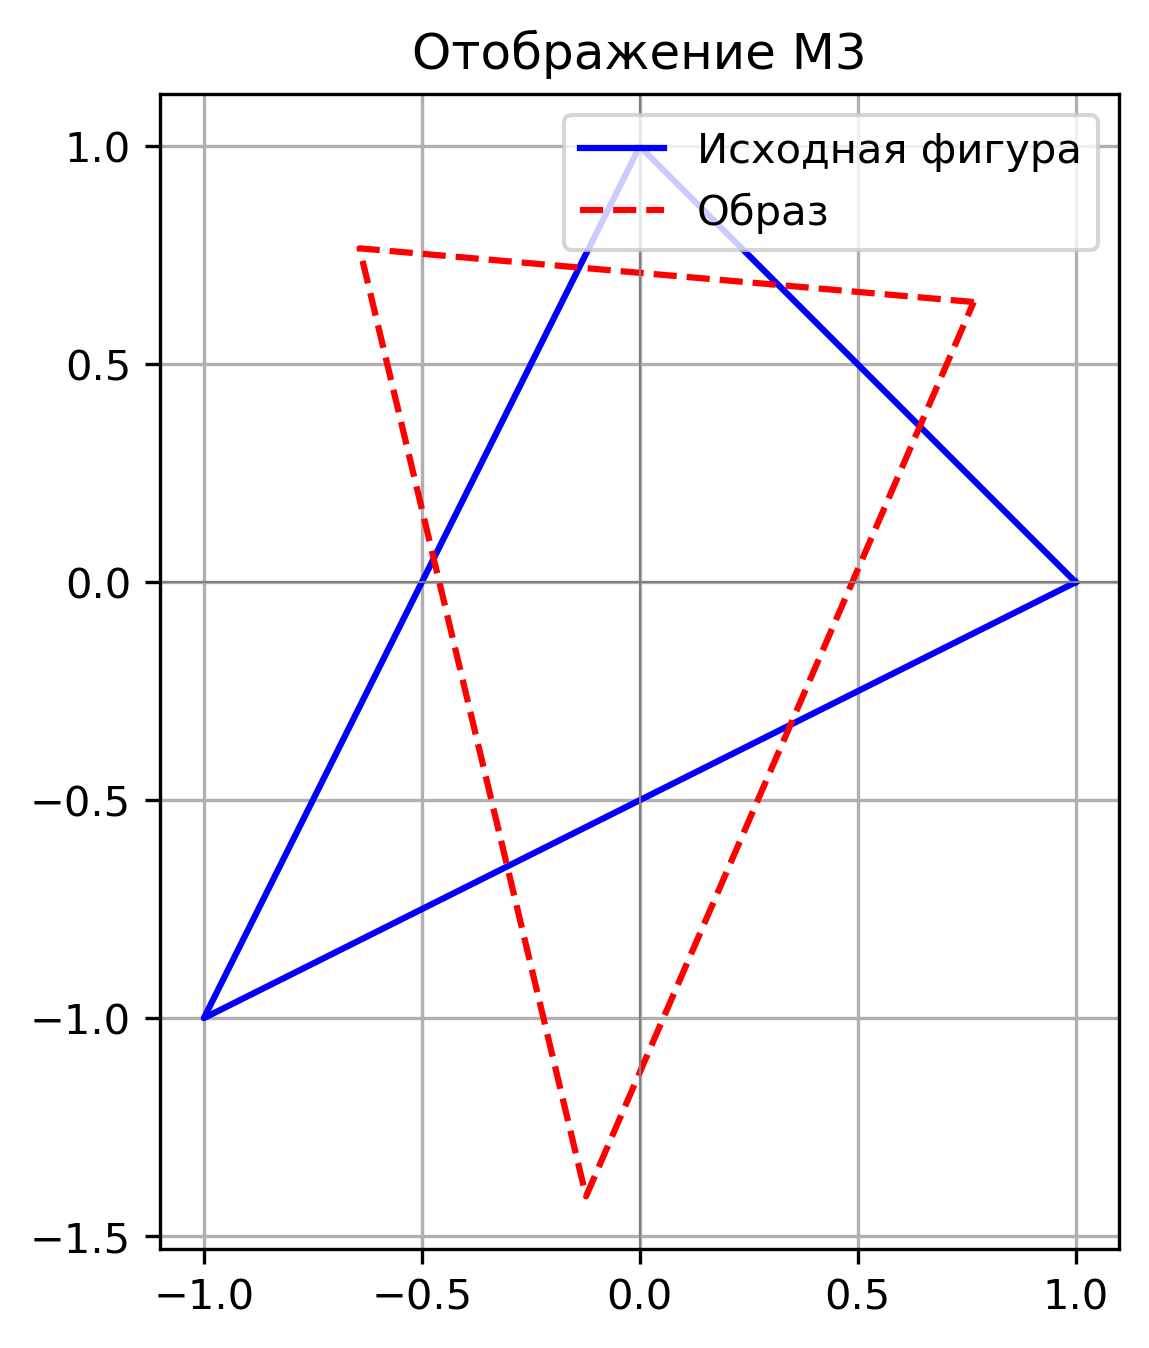
\includegraphics[width=\linewidth]{plots/M3.png}
    \caption{$M_3$}
  \end{subfigure}

  \vspace{0.5cm}

  \begin{subfigure}[b]{0.3\textwidth}
    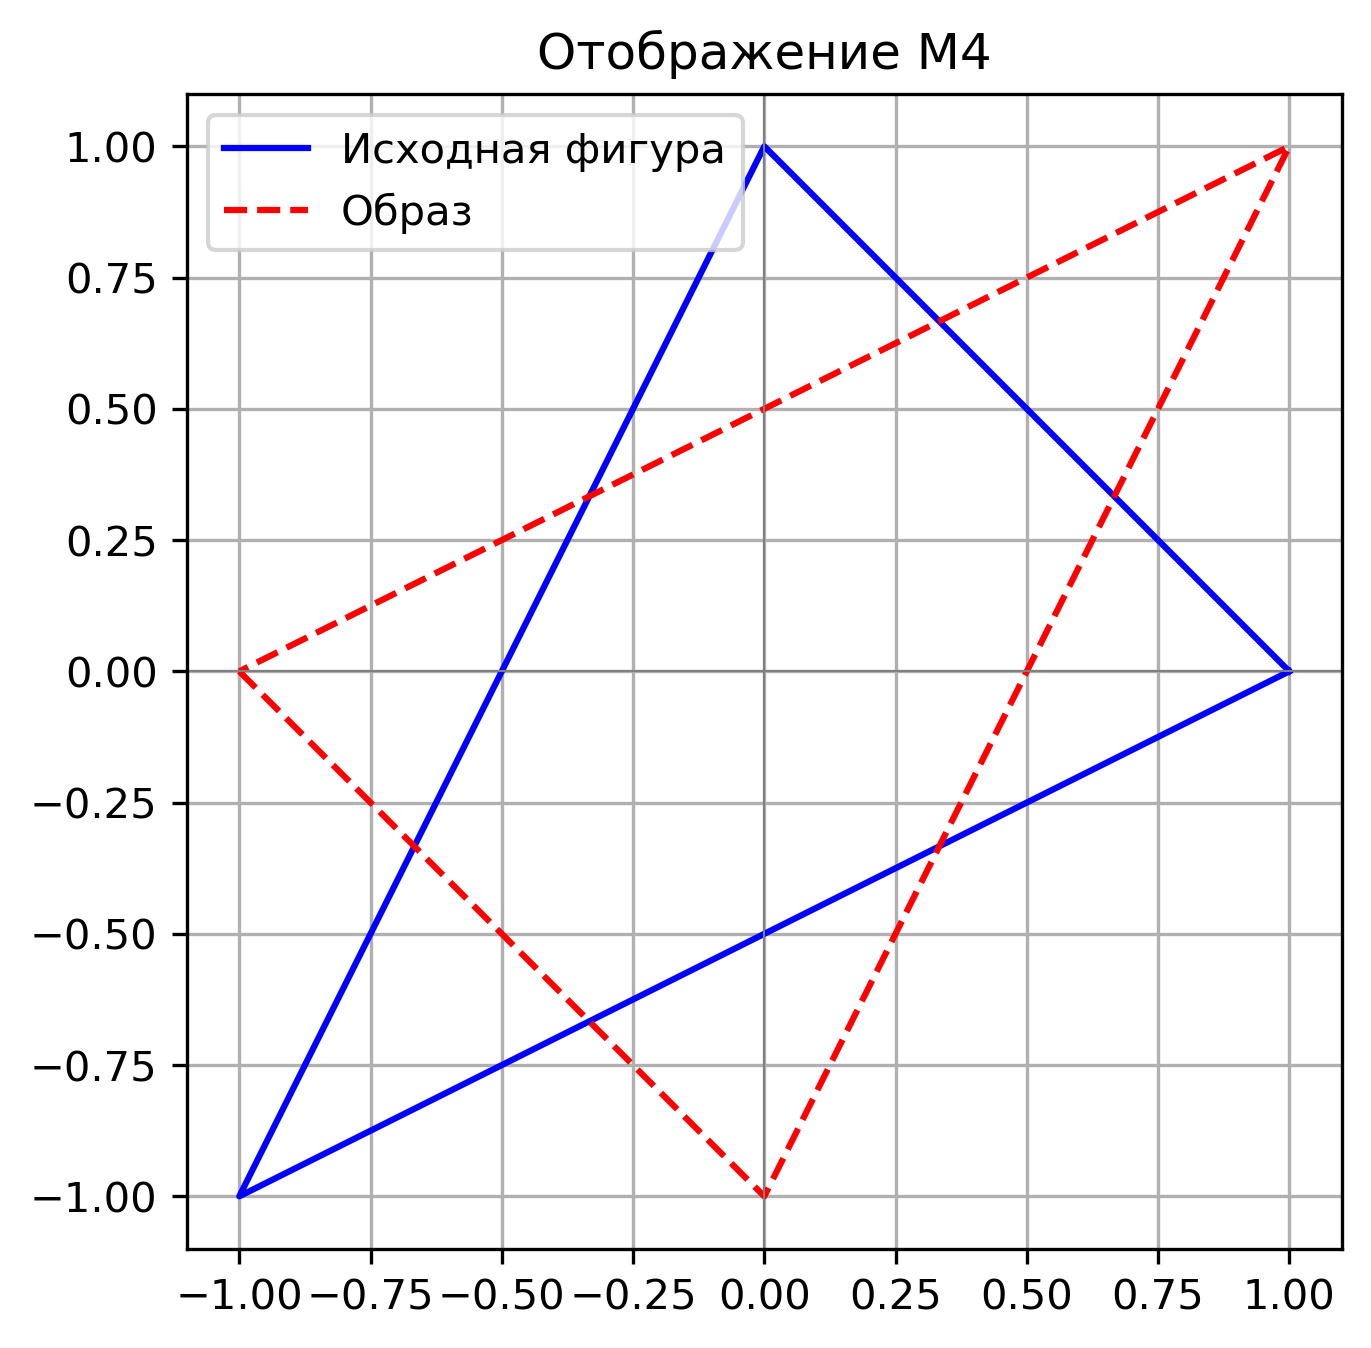
\includegraphics[width=\linewidth]{plots/M4.png}
    \caption{$M_4$}
  \end{subfigure}\hfill
  \begin{subfigure}[b]{0.3\textwidth}
    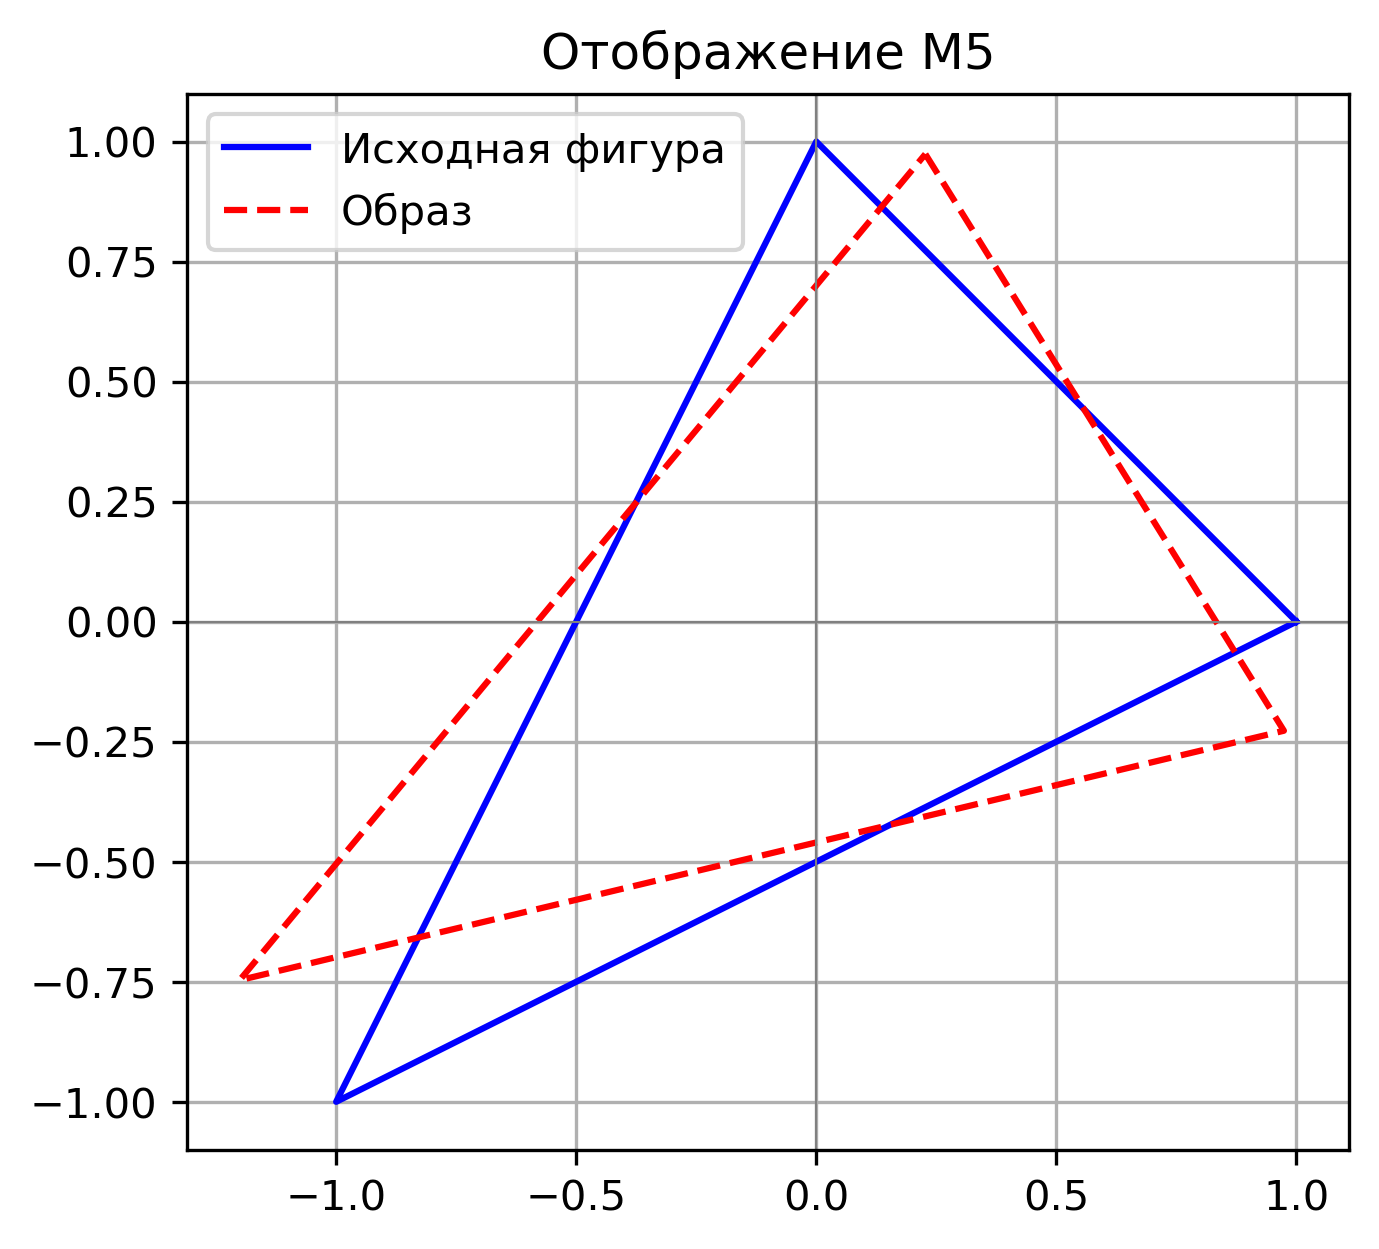
\includegraphics[width=\linewidth]{plots/M5.png}
    \caption{$M_5$}
  \end{subfigure}\hfill
  \begin{subfigure}[b]{0.3\textwidth}
    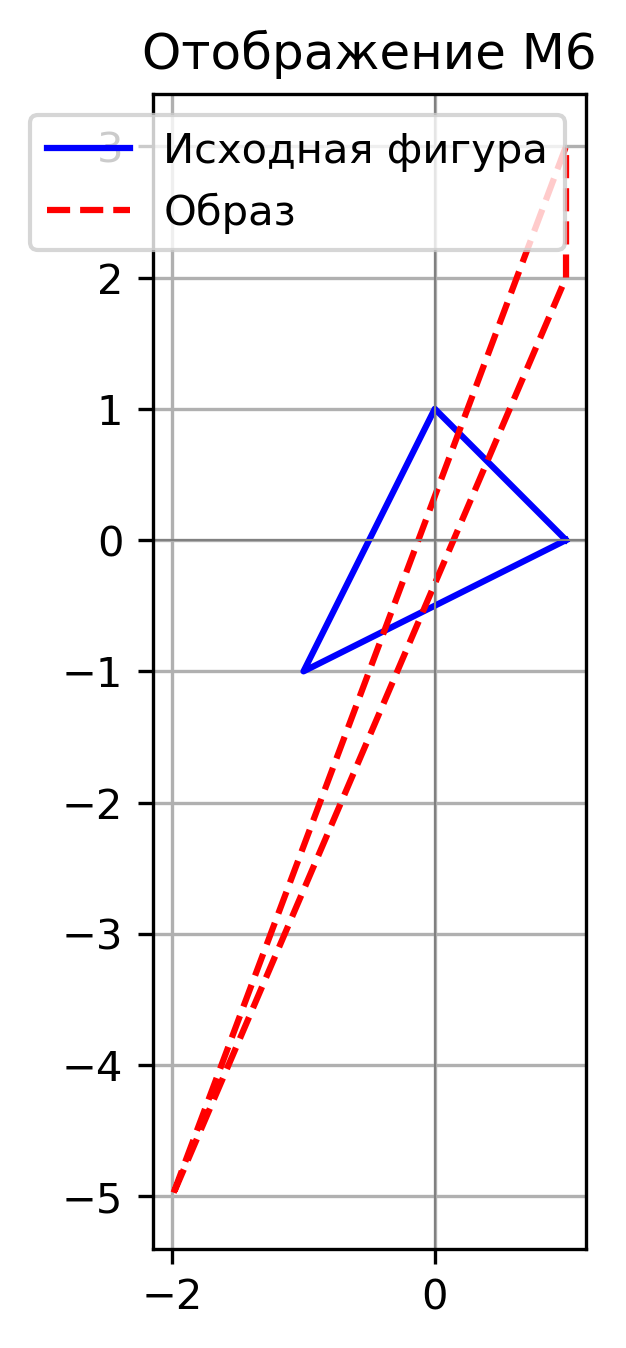
\includegraphics[width=\linewidth]{plots/M6.png}
    \caption{$M_6$}
  \end{subfigure}
  \caption{Отображения $M_1$–$M_6$}
\end{figure}

\clearpage

\begin{figure}[H]
  \centering
  \begin{subfigure}[b]{0.3\textwidth}
    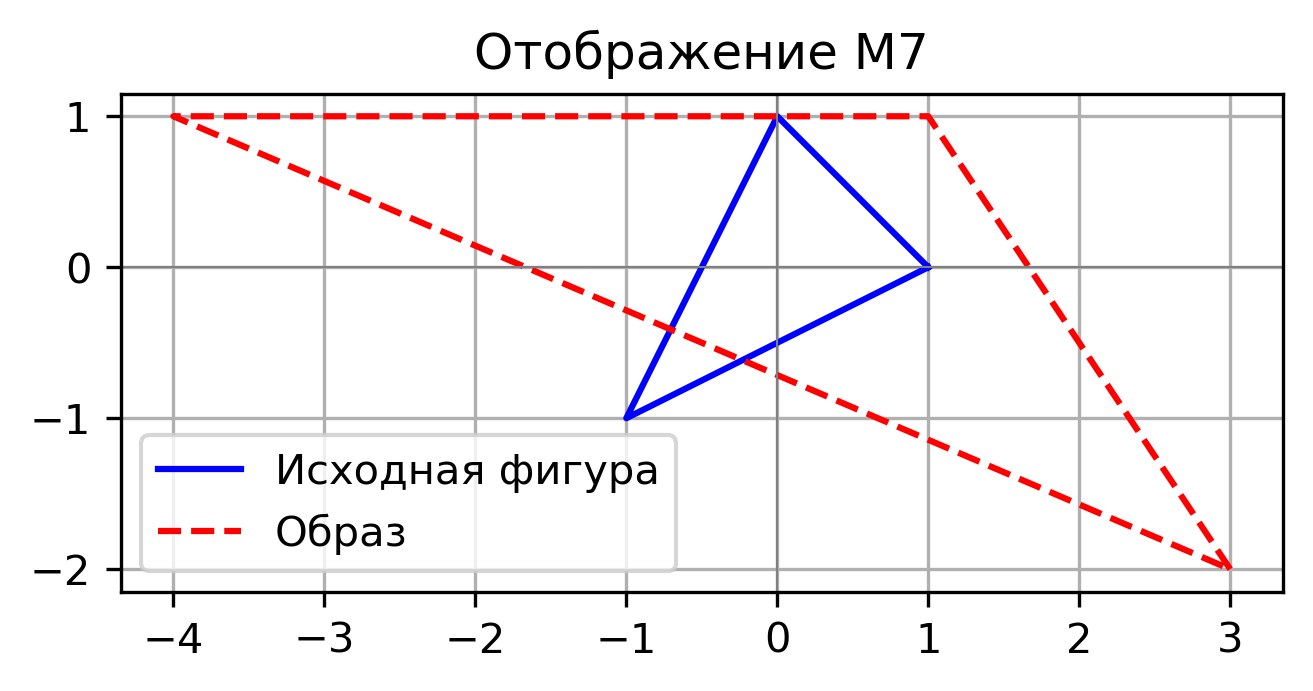
\includegraphics[width=\linewidth]{plots/M7.png}
    \caption{$M_7$}
  \end{subfigure}\hfill
  \begin{subfigure}[b]{0.3\textwidth}
    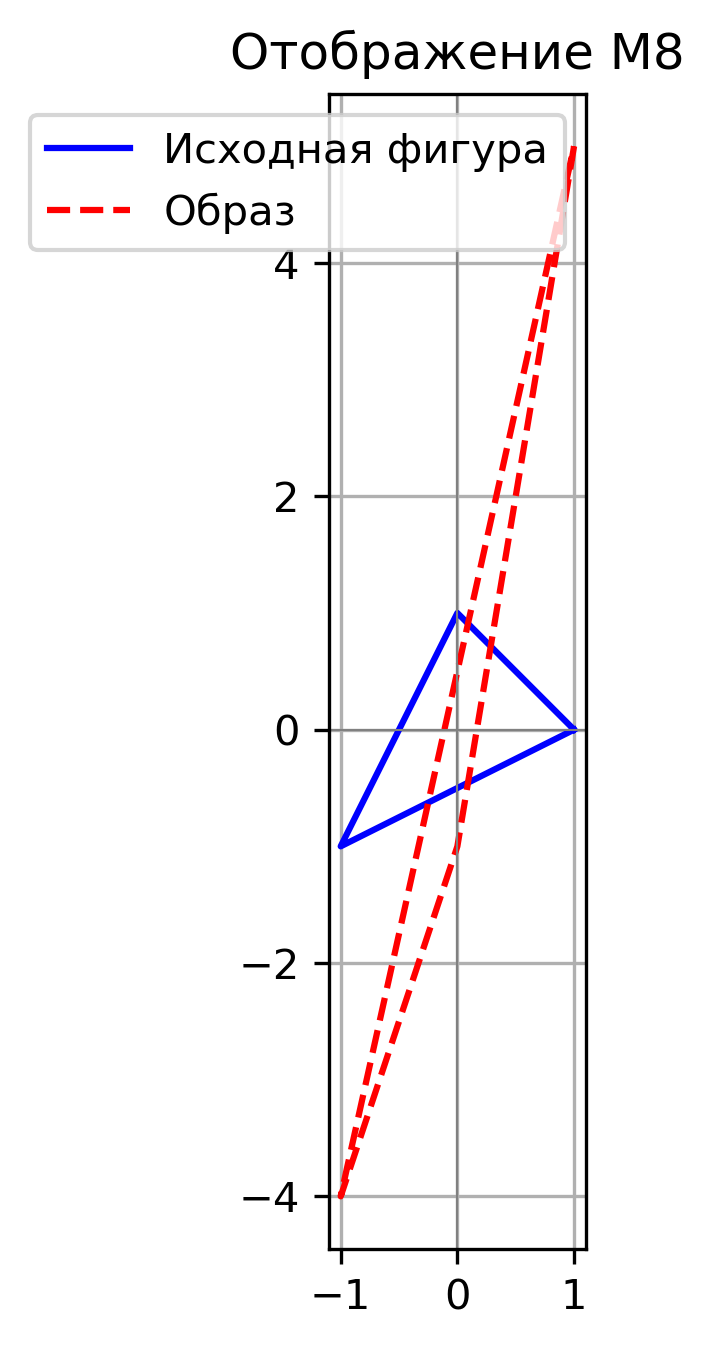
\includegraphics[width=\linewidth]{plots/M8.png}
    \caption{$M_8$}
  \end{subfigure}\hfill
  \begin{subfigure}[b]{0.3\textwidth}
    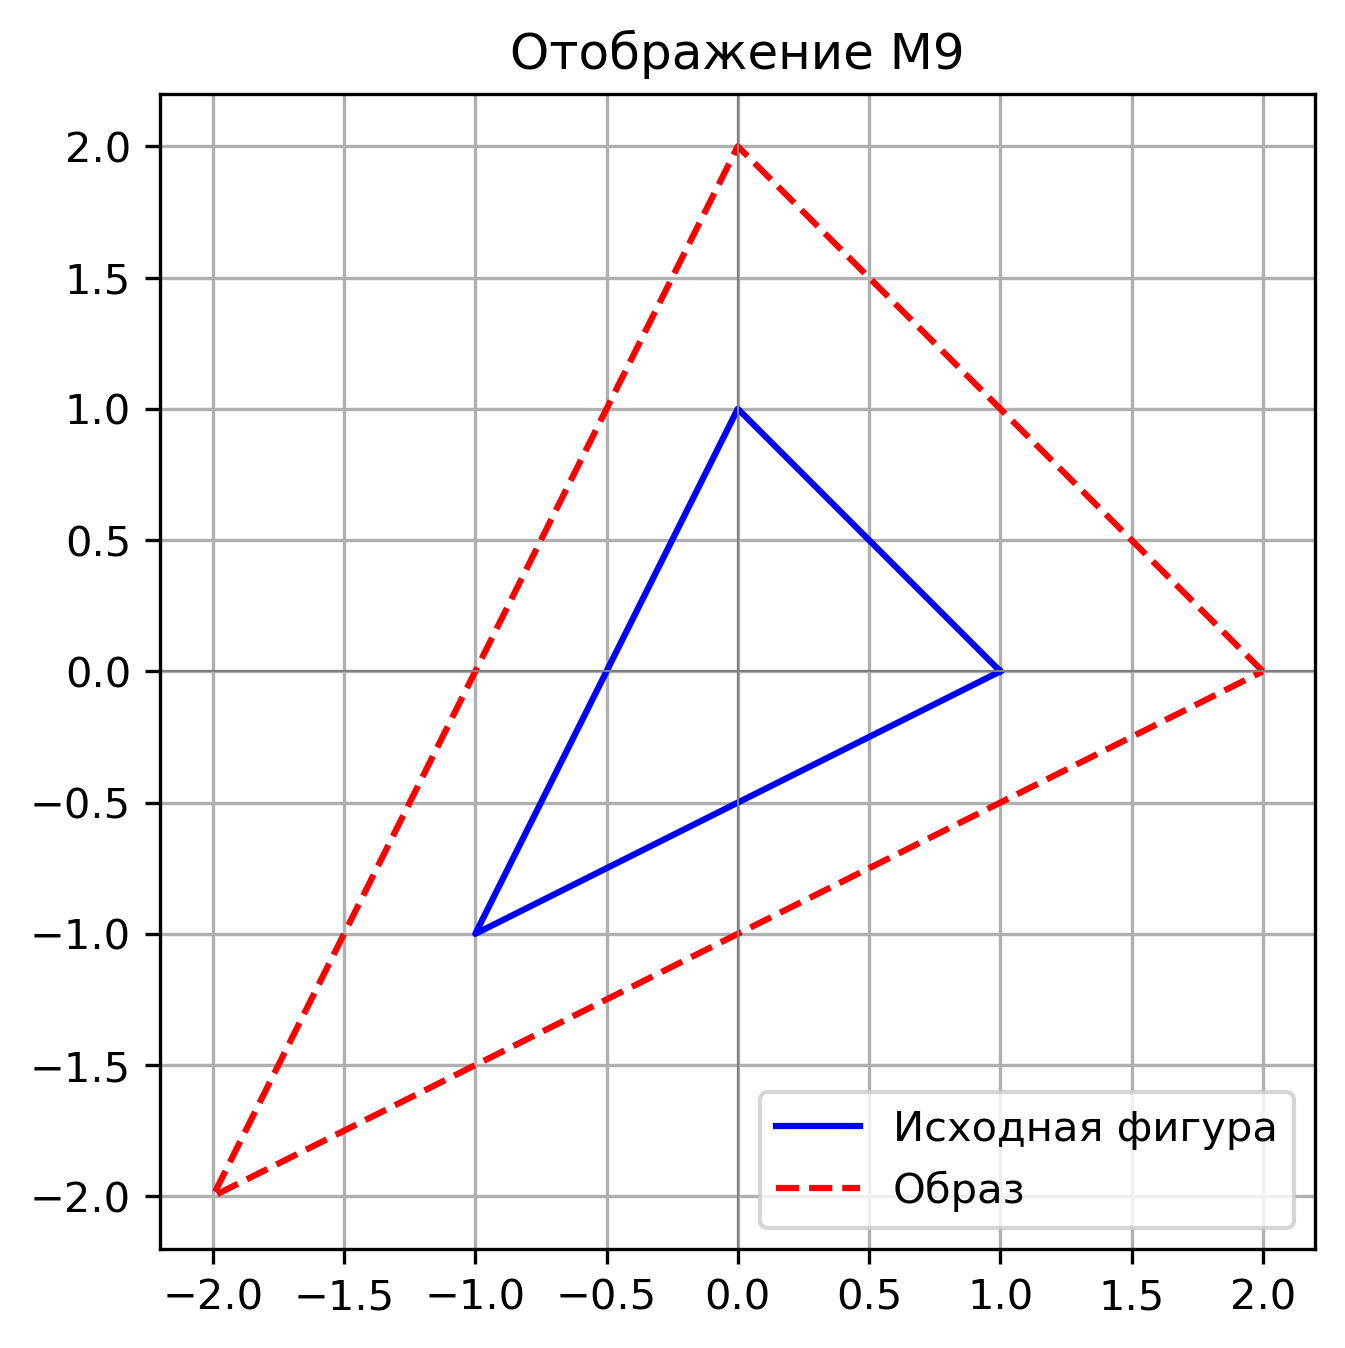
\includegraphics[width=\linewidth]{plots/M9.png}
    \caption{$M_9$}
  \end{subfigure}

  \vspace{0.5cm}

  \begin{subfigure}[b]{0.3\textwidth}
    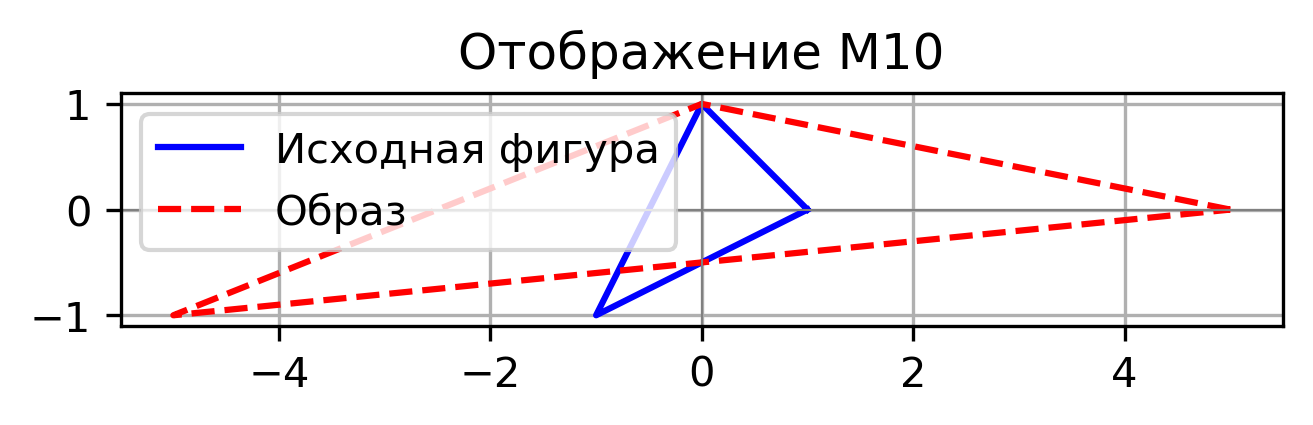
\includegraphics[width=\linewidth]{plots/M10.png}
    \caption{$M_{10}$}
  \end{subfigure}\hfill
  \begin{subfigure}[b]{0.3\textwidth}
    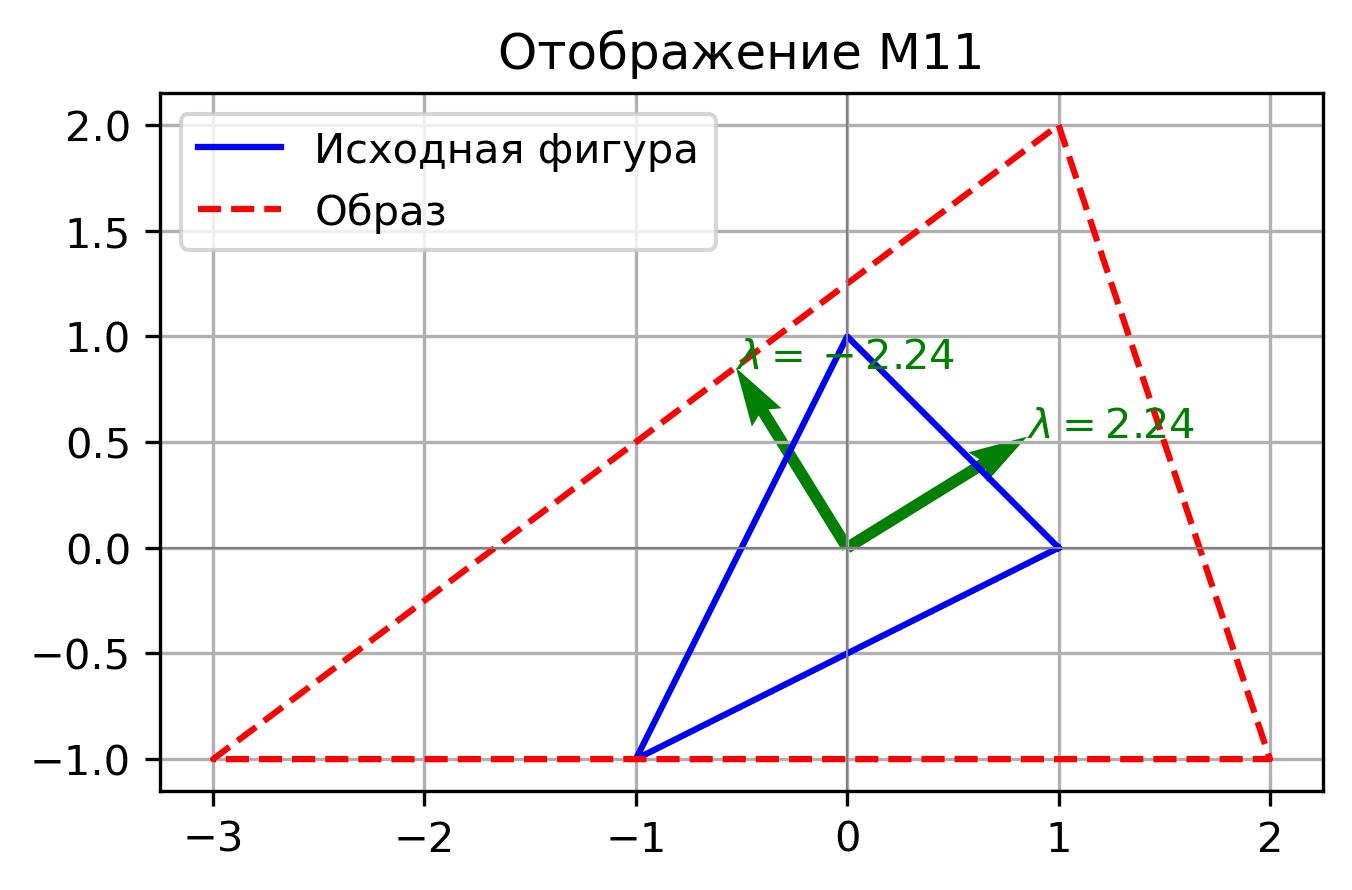
\includegraphics[width=\linewidth]{plots/M11.png}
    \caption{$M_{11}$}
  \end{subfigure}\hfill
  \begin{subfigure}[b]{0.3\textwidth}
    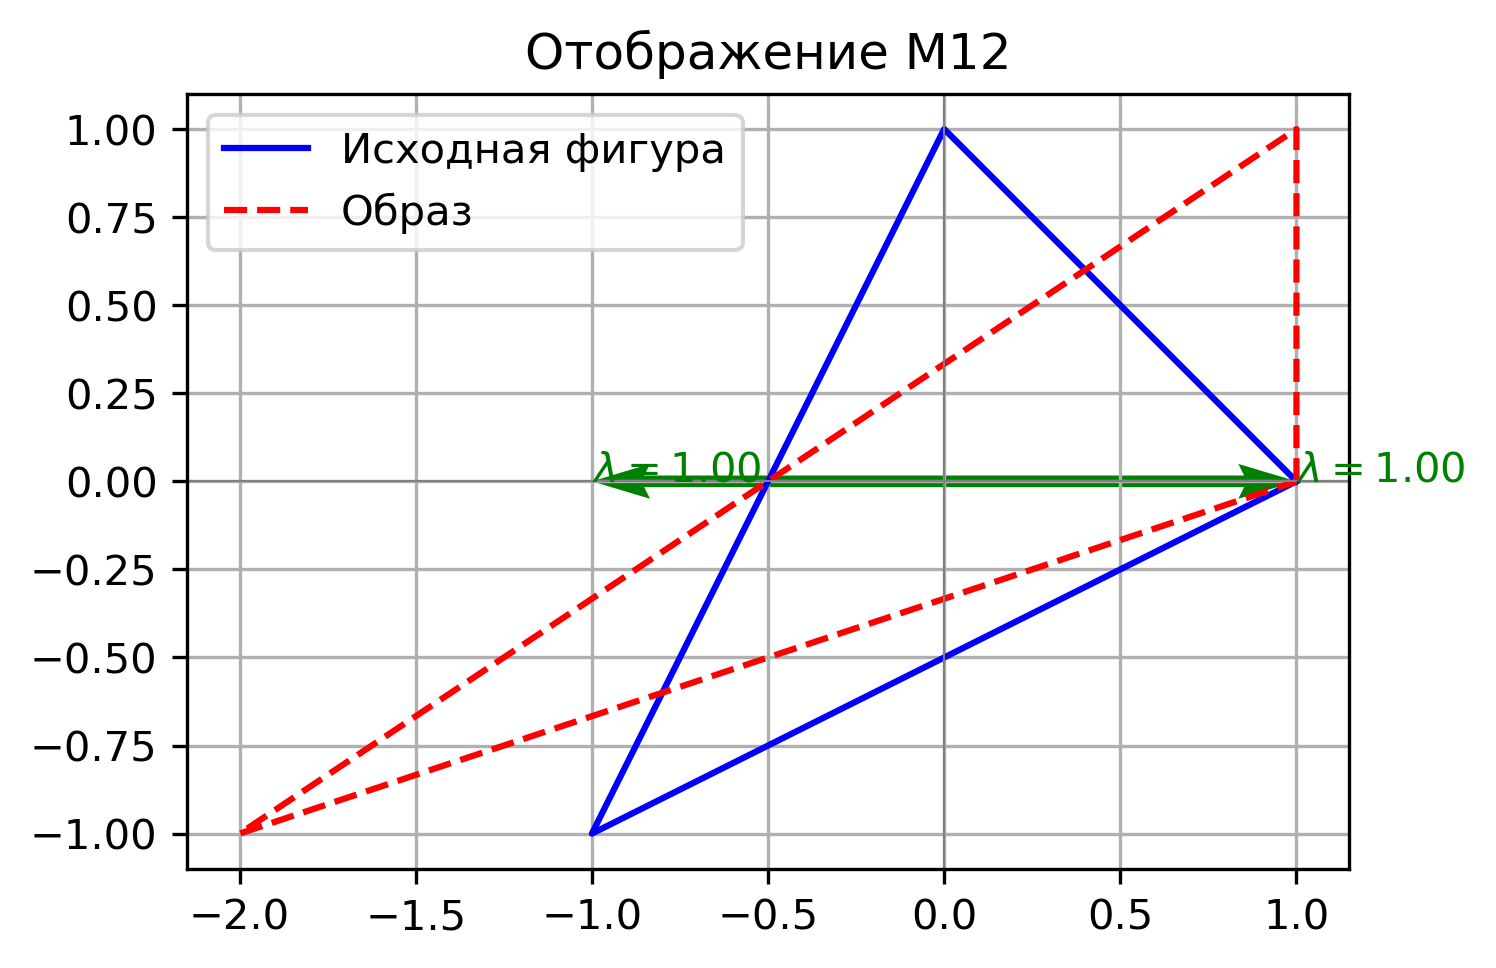
\includegraphics[width=\linewidth]{plots/M12.png}
    \caption{$M_{12}$}
  \end{subfigure}
  \caption{Отображения $M_7$–$M_{12}$}
\end{figure}

\begin{figure}[H]
  \centering
  \begin{subfigure}[b]{0.3\textwidth}
    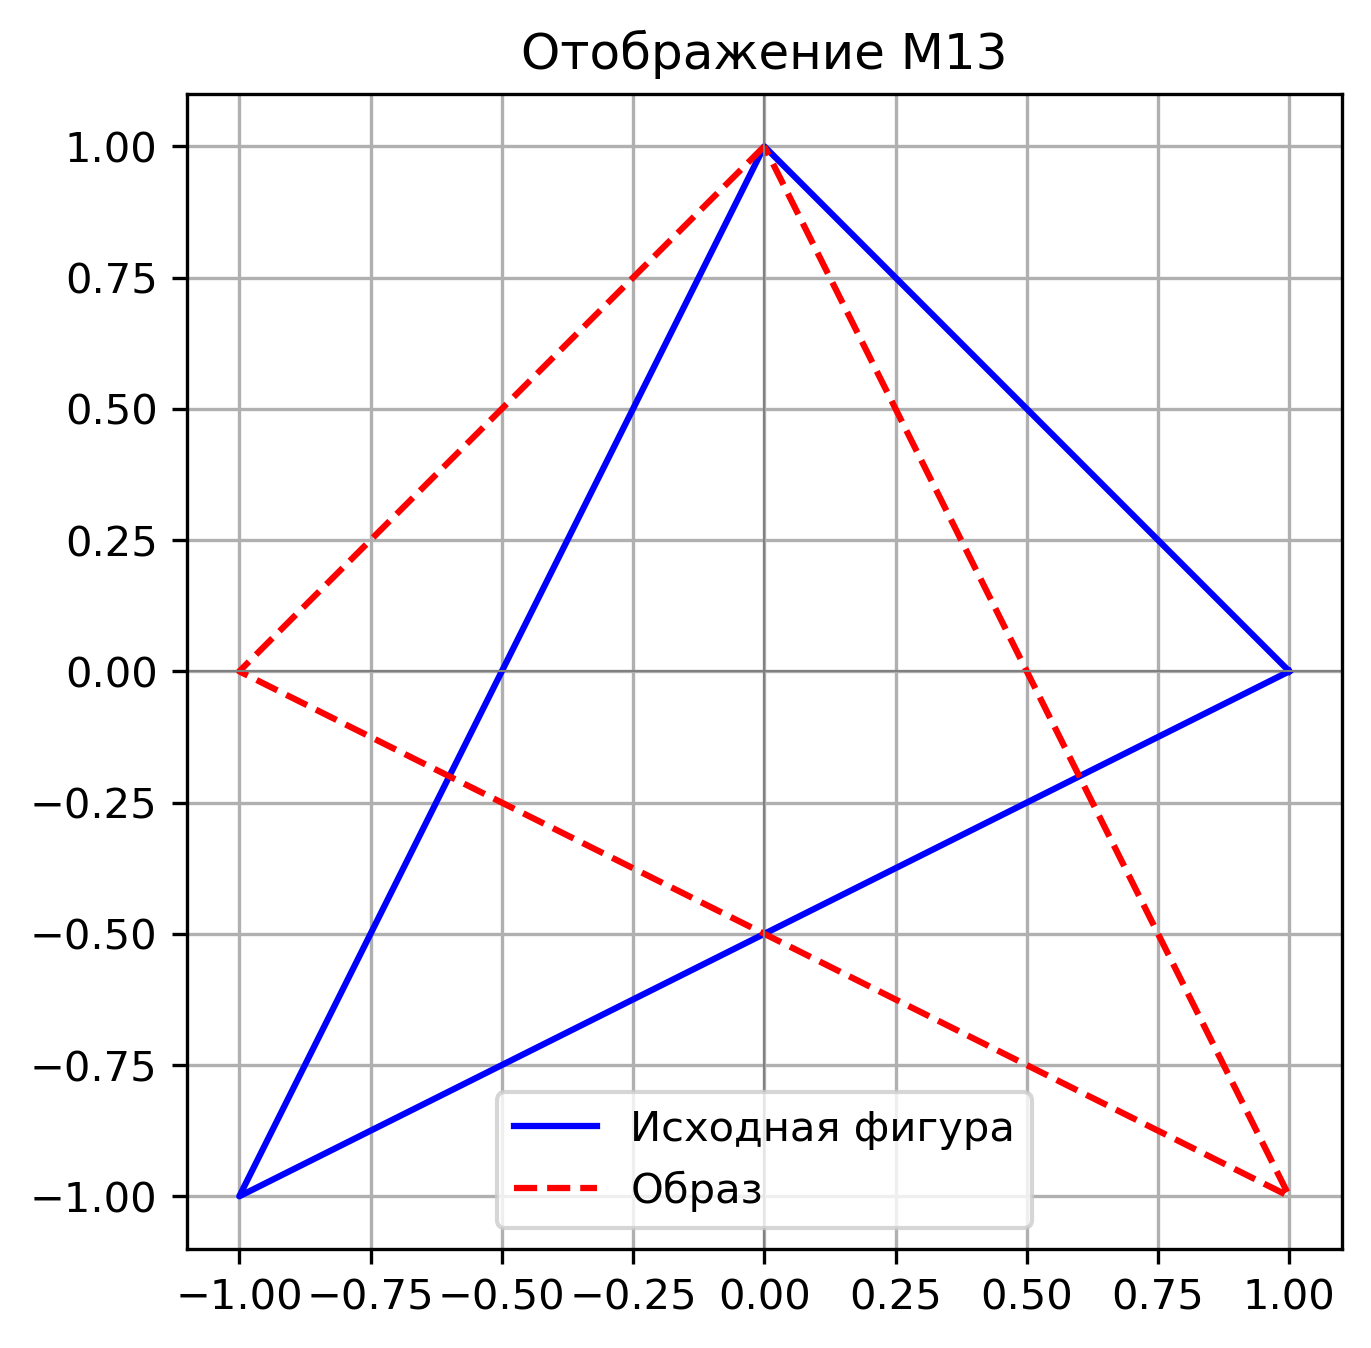
\includegraphics[width=\linewidth]{plots/M13.png}
    \caption{$M_{13}$}
  \end{subfigure}\hfill
  \begin{subfigure}[b]{0.3\textwidth}
    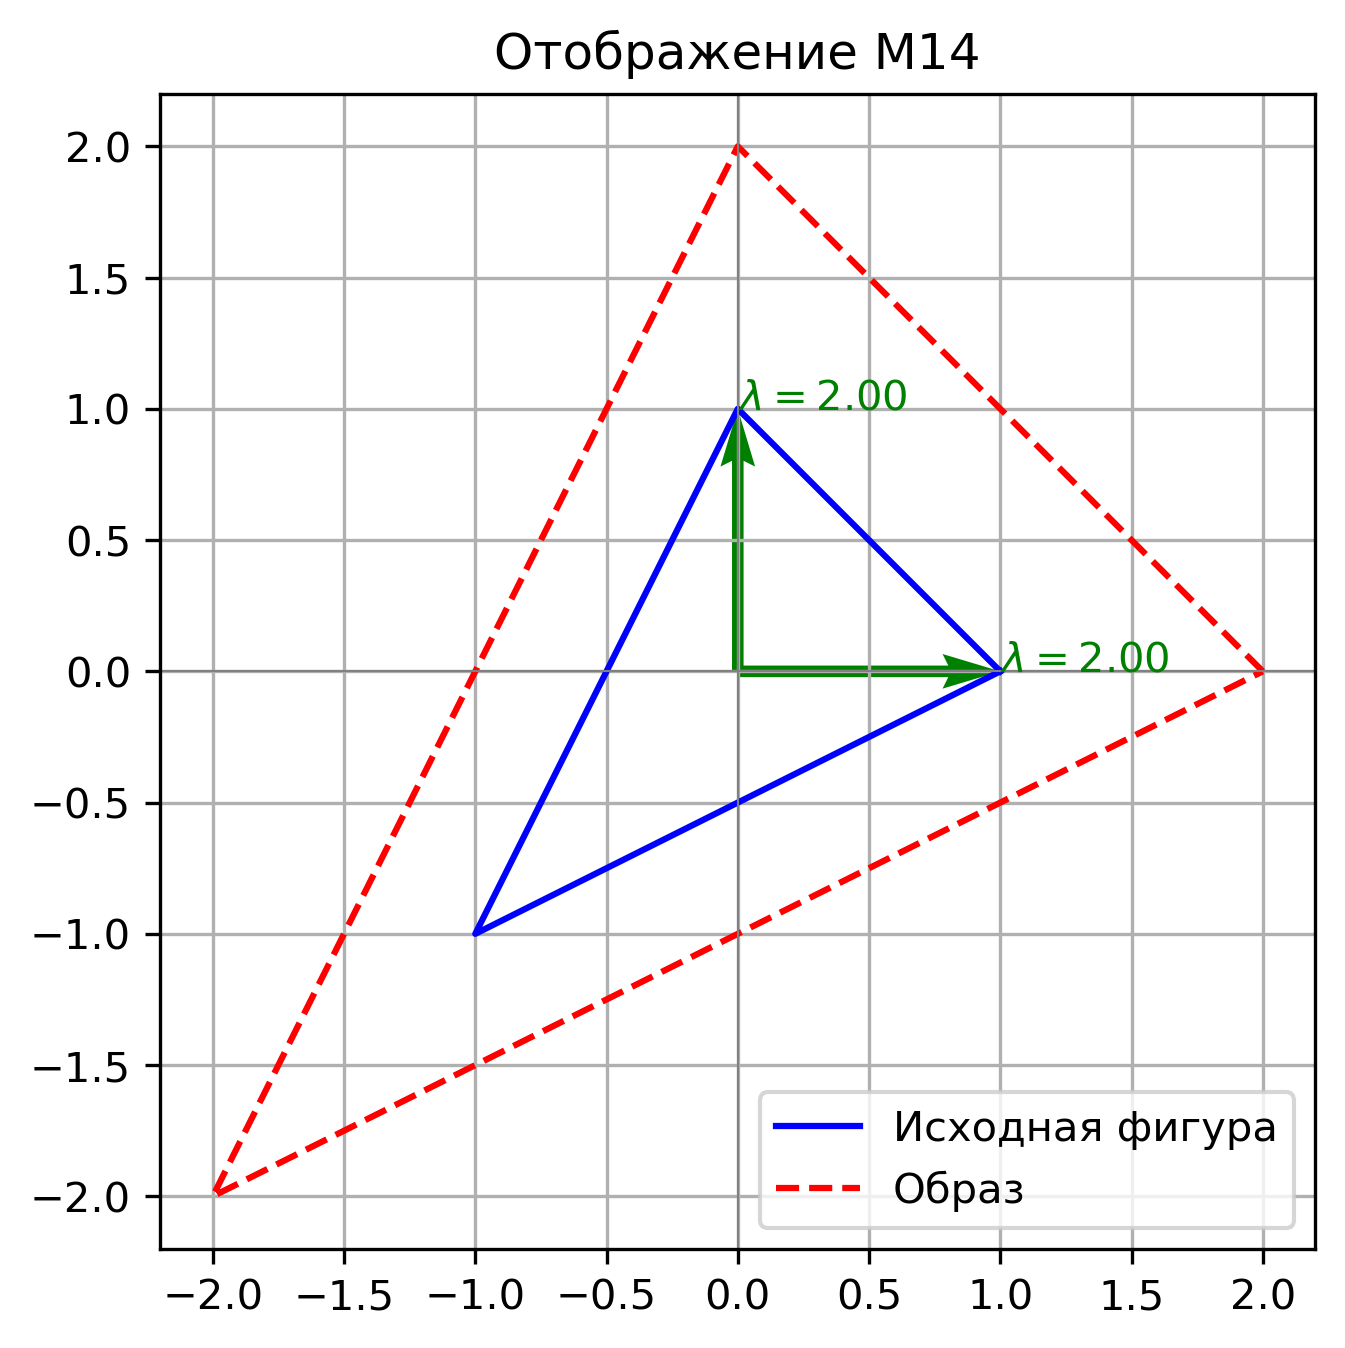
\includegraphics[width=\linewidth]{plots/M14.png}
    \caption{$M_{14}$}
  \end{subfigure}\hfill
  \begin{subfigure}[b]{0.3\textwidth}
    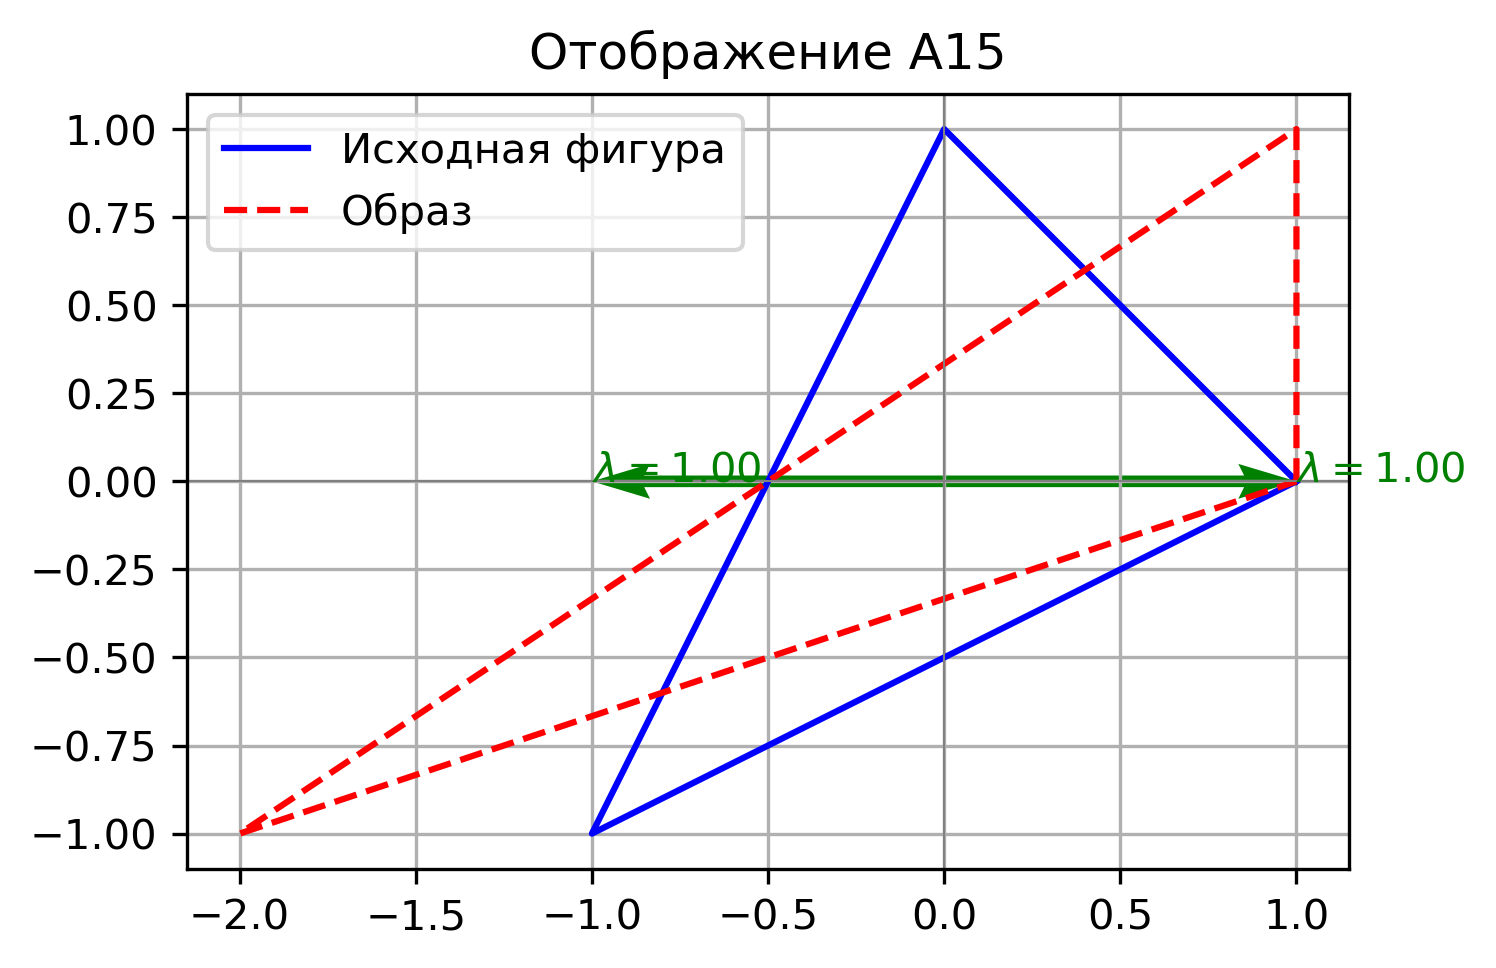
\includegraphics[width=\linewidth]{plots/A15.png}
    \caption{$A_{15}$}
  \end{subfigure}

  \vspace{0.5cm}

  \begin{subfigure}[b]{0.3\textwidth}
    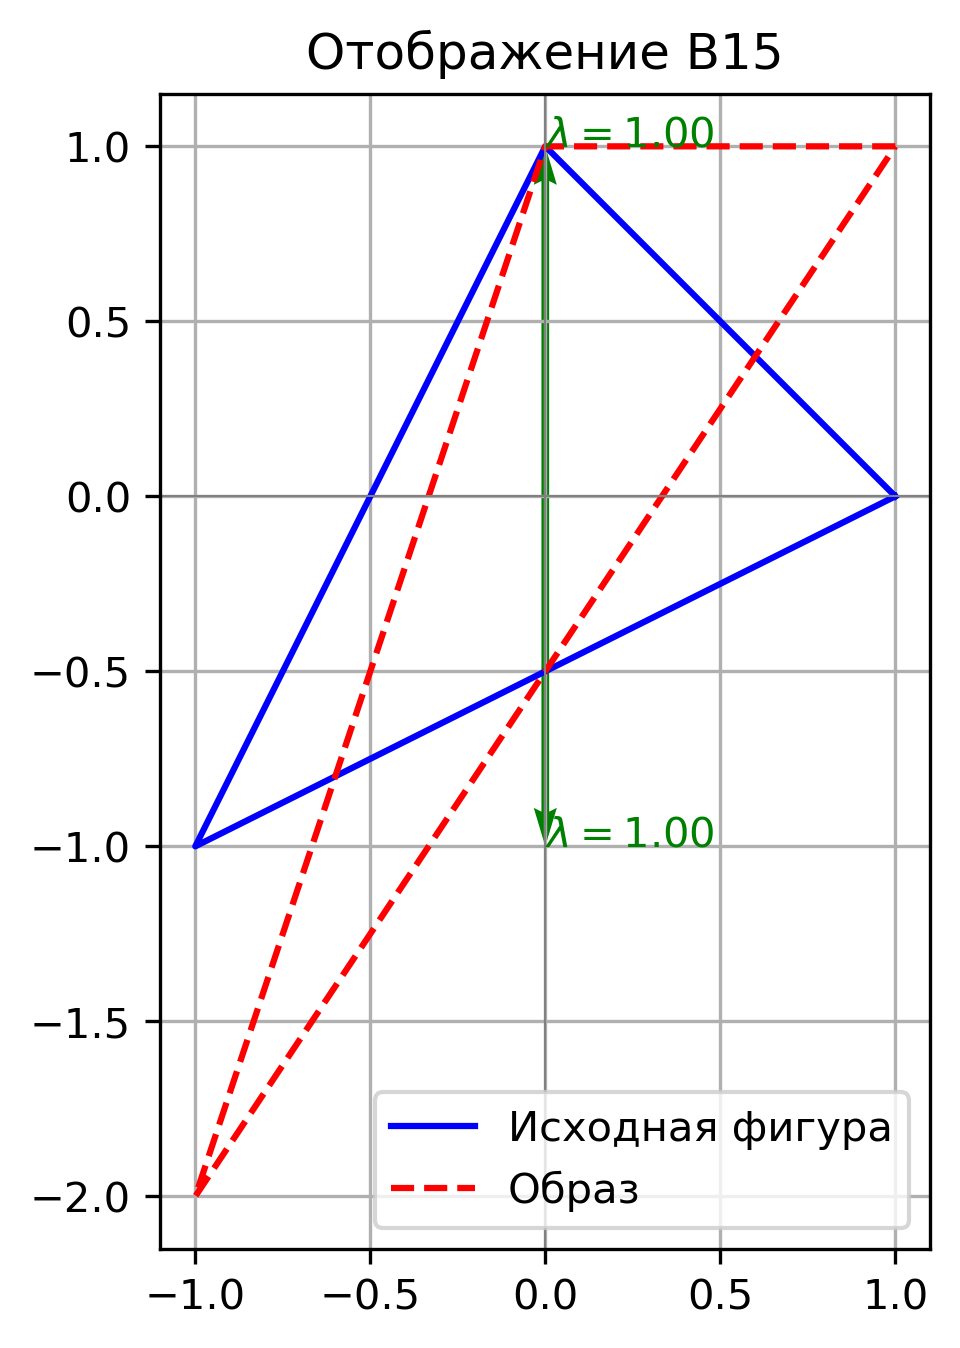
\includegraphics[width=\linewidth]{plots/B15.png}
    \caption{$B_{15}$}
  \end{subfigure}\hfill
  \begin{subfigure}[b]{0.3\textwidth}
    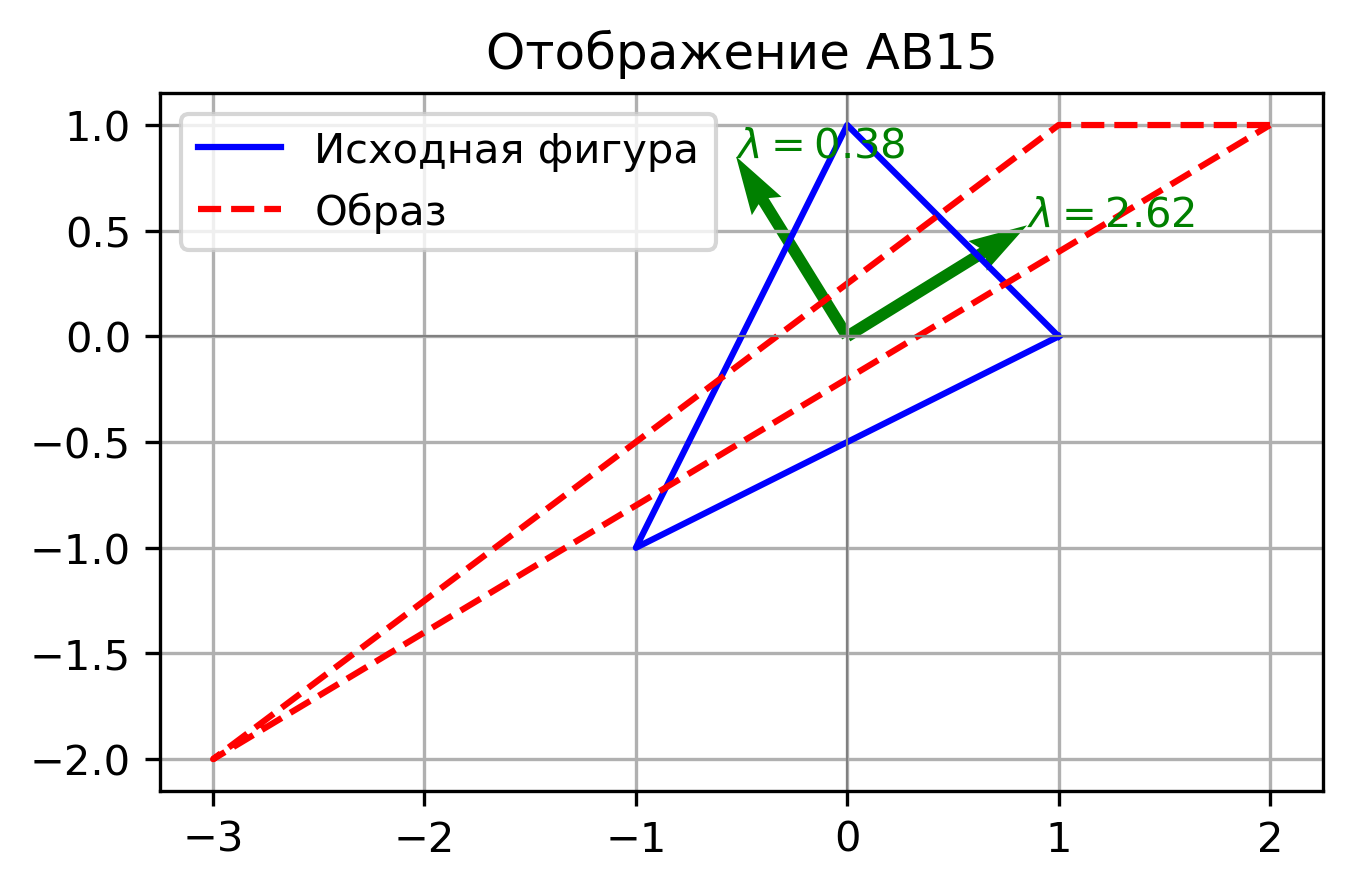
\includegraphics[width=\linewidth]{plots/AB15.png}
    \caption{$A_{15}B_{15}$}
  \end{subfigure}\hfill
  \begin{subfigure}[b]{0.3\textwidth}
    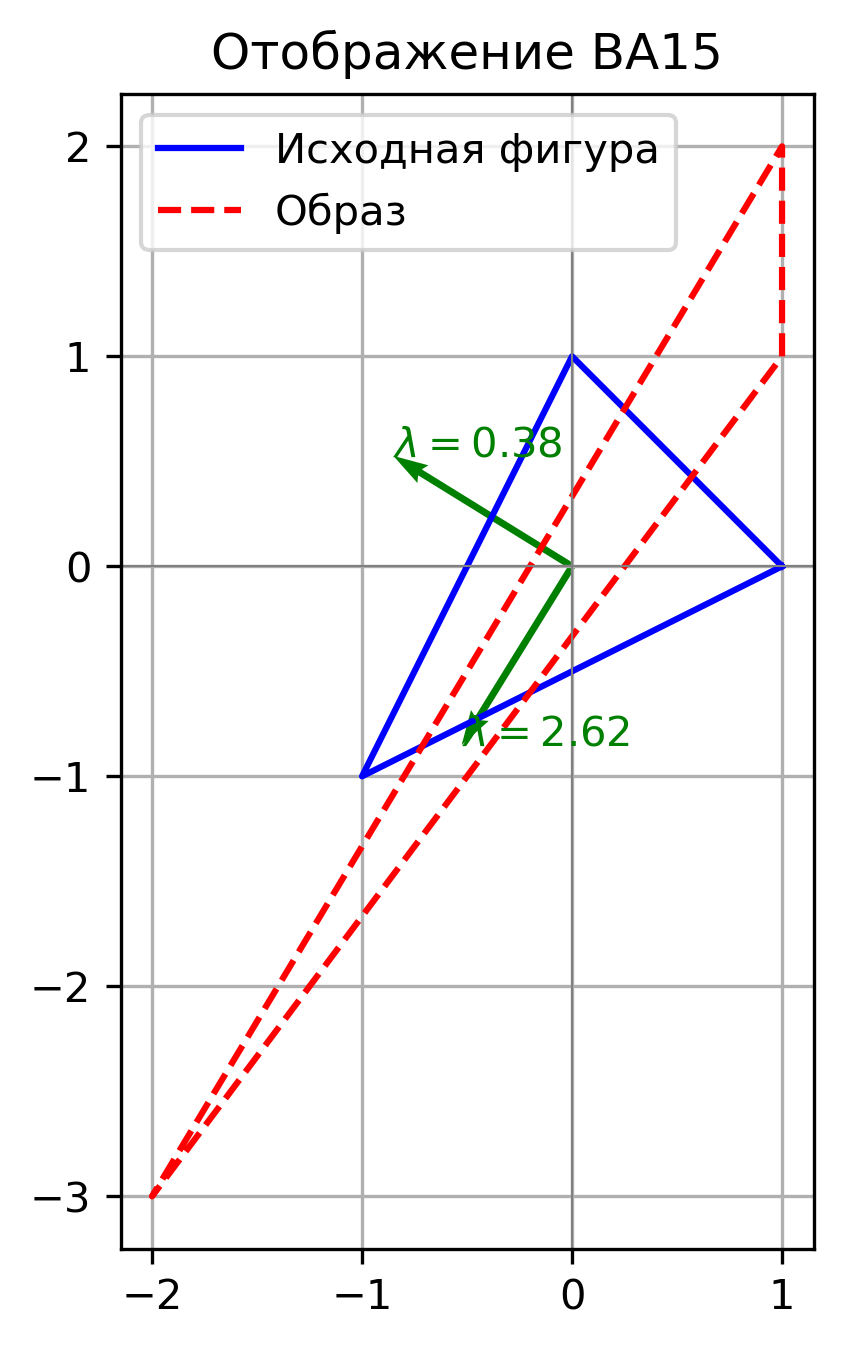
\includegraphics[width=\linewidth]{plots/BA15.png}
    \caption{$B_{15}A_{15}$}
  \end{subfigure}
  \caption{Отображения $M_{13}$–$BA_{15}$}
\end{figure}

\clearpage

\begin{figure}[H]
  \centering
  \begin{subfigure}[b]{0.3\textwidth}
    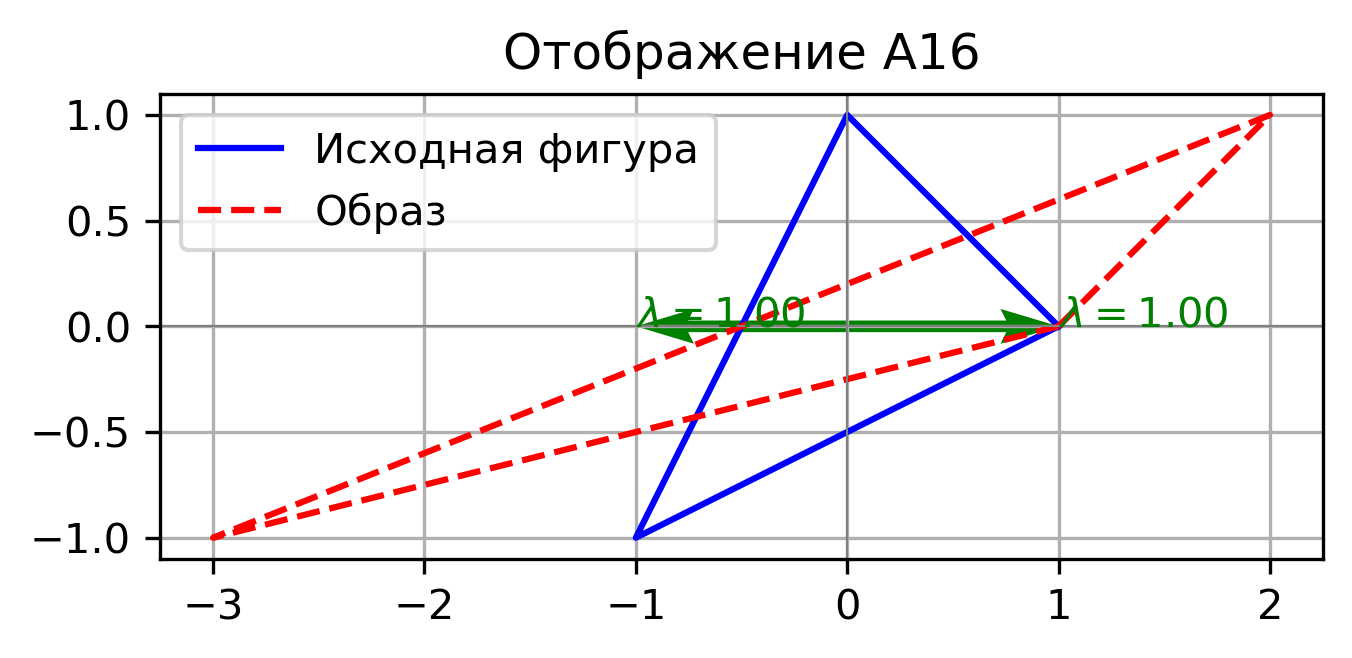
\includegraphics[width=\linewidth]{plots/A16.png}
    \caption{$A_{16}$}
  \end{subfigure}\hfill
  \begin{subfigure}[b]{0.3\textwidth}
    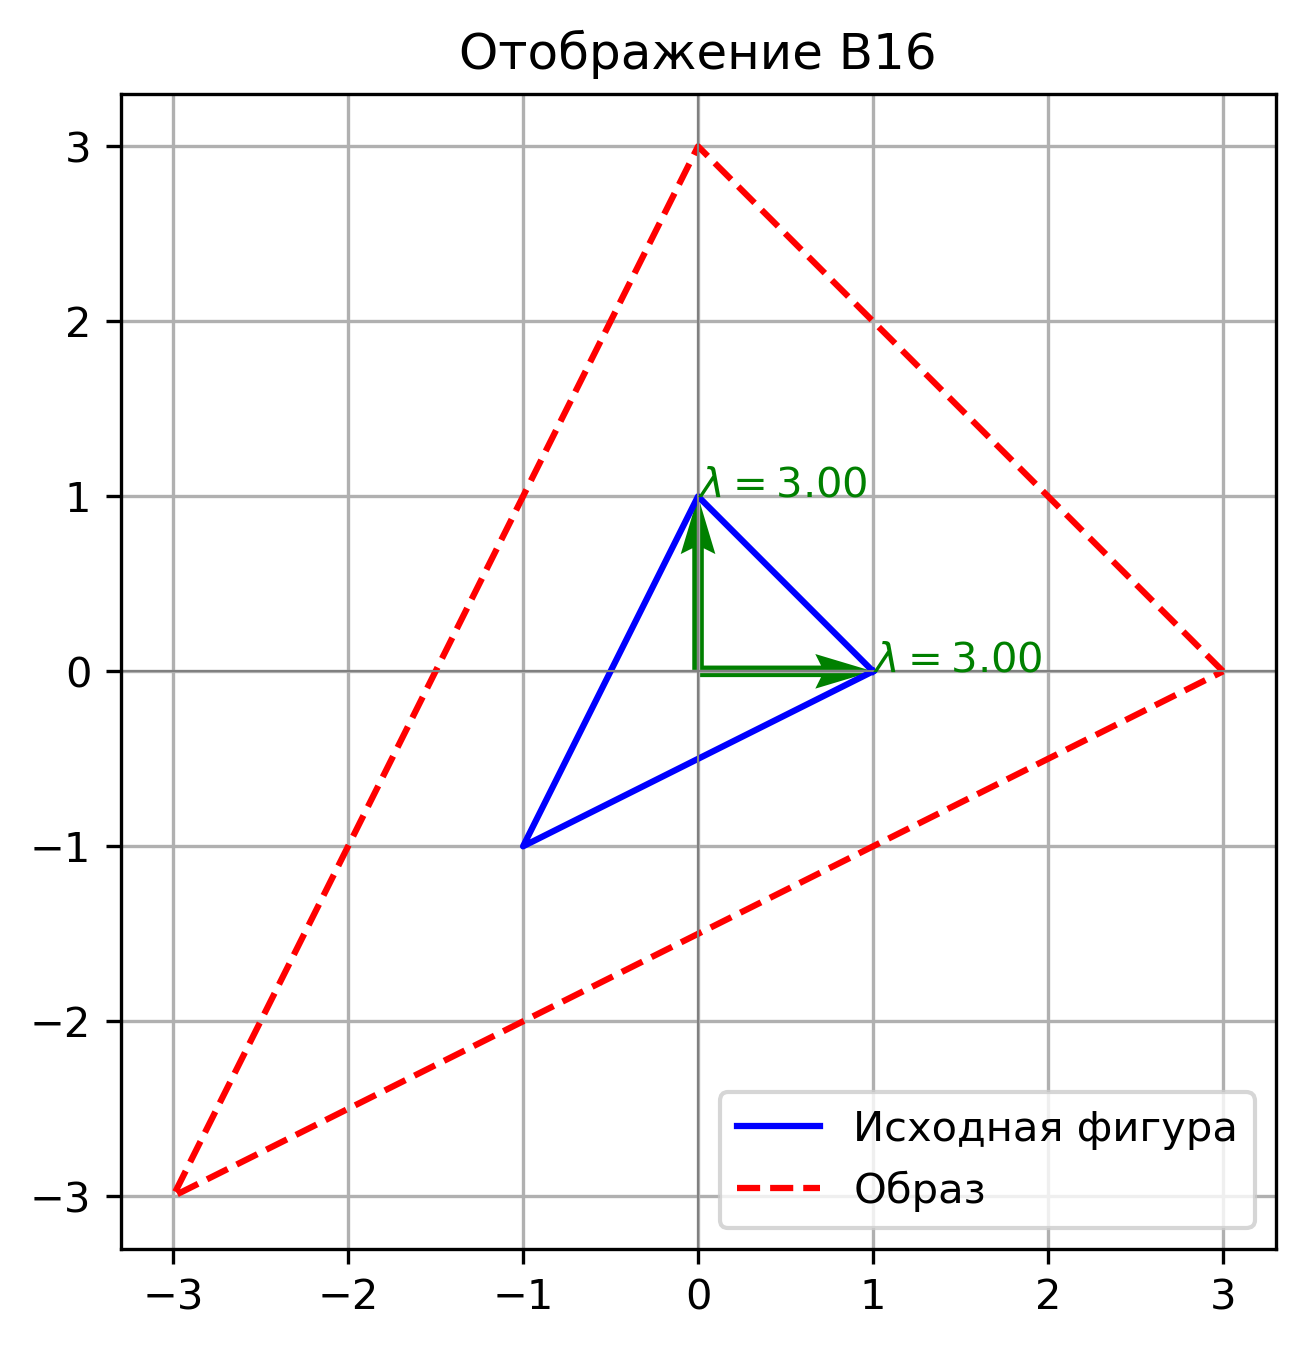
\includegraphics[width=\linewidth]{plots/B16.png}
    \caption{$B_{16}$}
  \end{subfigure}\hfill
  \begin{subfigure}[b]{0.3\textwidth}
    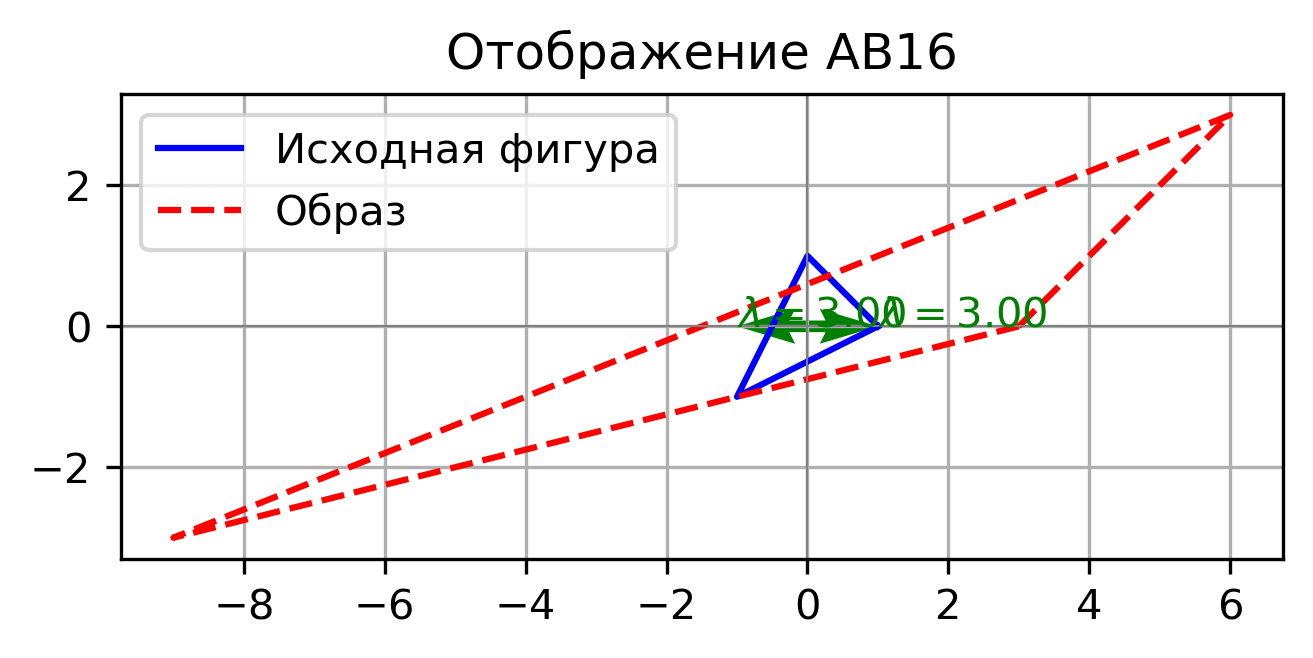
\includegraphics[width=\linewidth]{plots/AB16.png}
    \caption{$A_{16}B_{16}$}
  \end{subfigure}

  \vspace{0.5cm}

  \begin{subfigure}[b]{0.3\textwidth}
    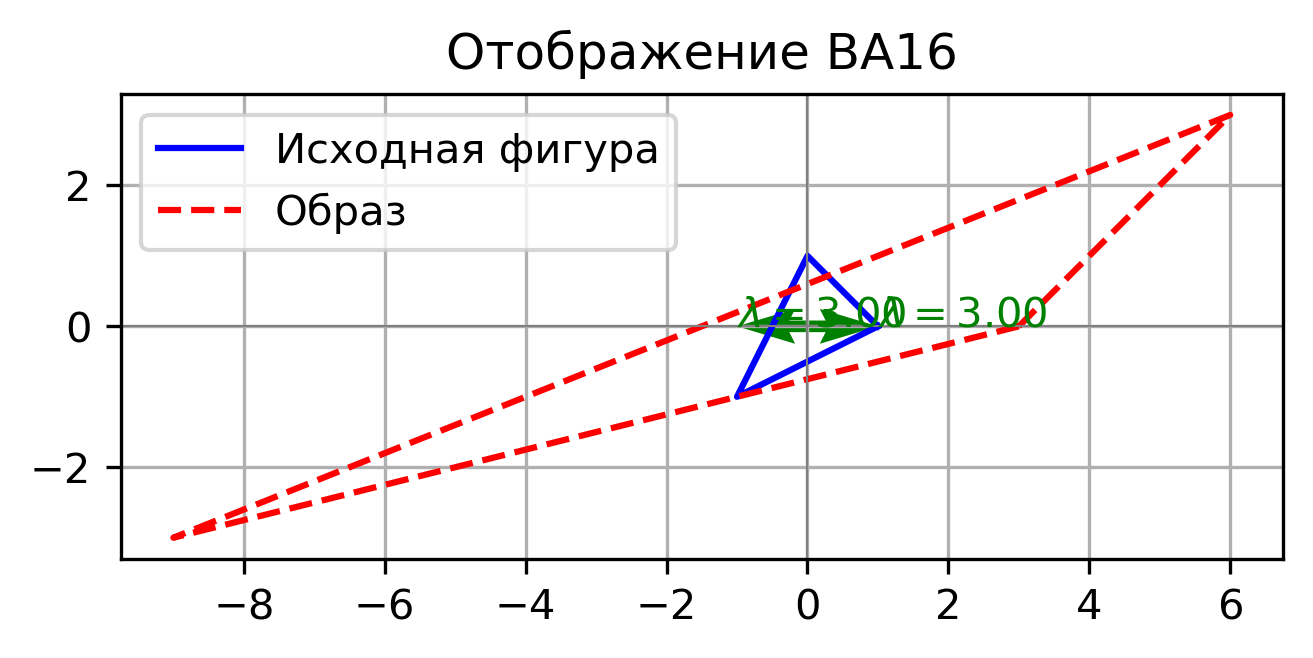
\includegraphics[width=\linewidth]{plots/BA16.png}
    \caption{$B_{16}A_{16}$}
  \end{subfigure}
  \caption{Отображения $A_{16}$–$BA_{16}$}
\end{figure}

\clearpage

% --- Краткие выводы ---
\section*{Выводы}
В работе сконструированы и проанализированы 2D-линейные преобразования, реализующие множество геометрических эффектов: отражения, проекции в прямую, повороты, изотропные и анизотропные масштабирующие отображения, а также примеры некомутации и коммутативности. Для каждого класса даны построения по геометрическим условиям (через образы базисных векторов, ортогональные разложения и жордановы формы), вычислены спектры, образы/ядра и определители. Показано, что симметричность матрицы \emph{обязательна} лишь для отражений через прямую, центральной симметрии, преобразований с ортогональным базисом собственных векторов и скалярных матриц; в остальных случаях она необязательна.